\begin{figure}[t]
    \centering
    \begin{minipage}[b]{0.63\linewidth}
        \centering
        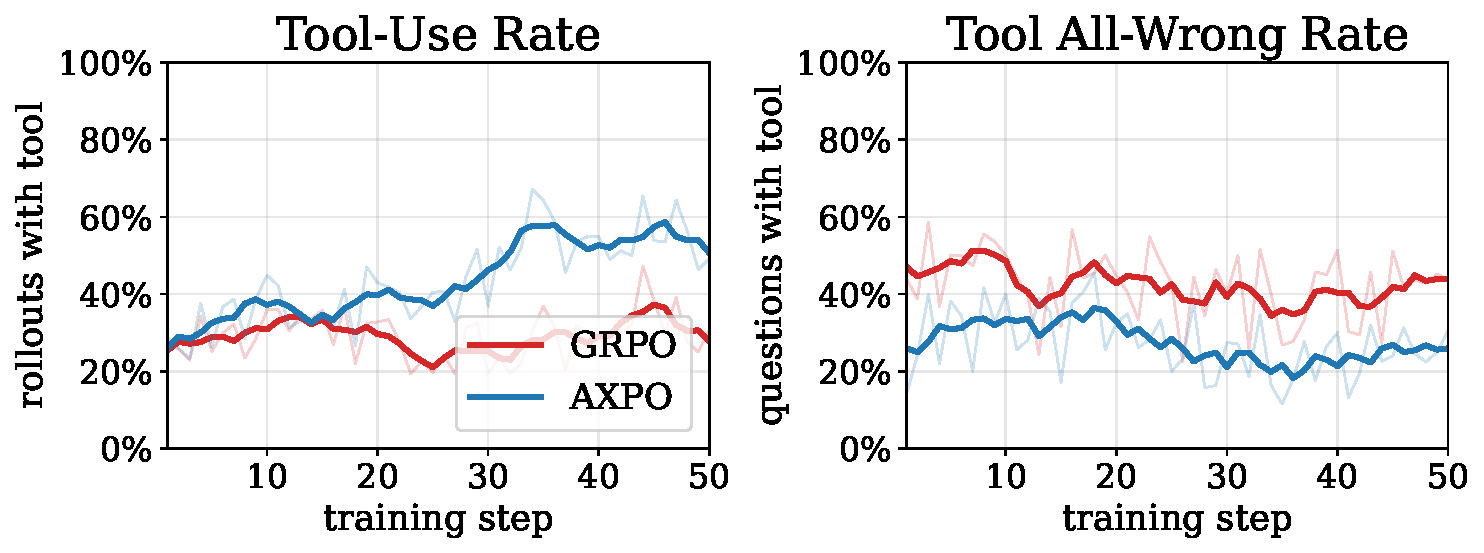
\includegraphics[width=\linewidth]{figures/fig4_training_dynamics_axpo_vs_grpo.pdf}
    \end{minipage}
    \begin{minipage}[b]{0.34\linewidth}
        \centering
        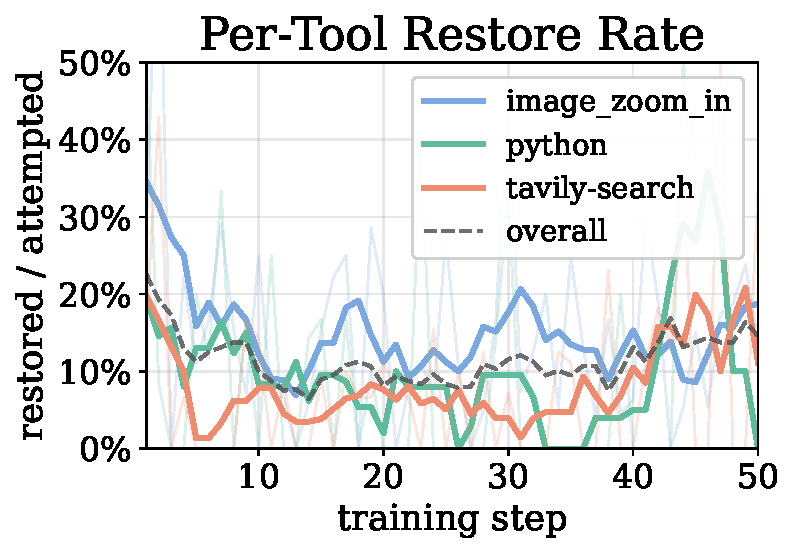
\includegraphics[width=\linewidth]{figures/fig4_per_tool_rescue.pdf}
    \end{minipage}
    \vspace{-0.1in}
    \caption{Both \gap symptoms reverse during AXPO training but stay flat under GRPO, and the recovery does happen at resampling. \textbf{Left \& Middle:} tool-use rate (top) and all-wrong rate on tool-using subgroups (bottom) over RL steps. \textbf{Right:} per-tool failed-subgroup recovery rate --- the share of all-wrong tool-using subgroups that resampling flips into a subgroup with at least one correct tool-using trajectory.}
    \vspace{-0.15in}
    \label{fig:training-dynamics}
\end{figure}

\begin{figure}[t]
    \centering
    \begin{subfigure}[b]{0.38\linewidth}
        \centering
        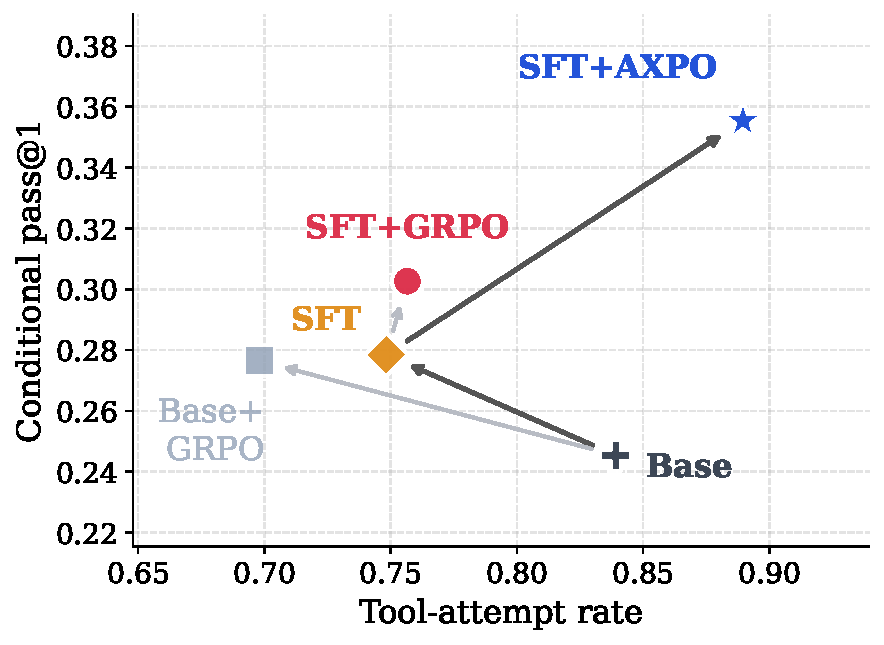
\includegraphics[width=\linewidth]{figures/figx_tool_calibration.pdf}
        \vspace{-0.15in}
        \caption{Training stages on the tool-attempt rate vs. conditional pass@1 plane. Only AXPO expands both axes simultaneously.}
        \label{fig:tool-calibration}
    \end{subfigure}\hfill
    \begin{subfigure}[b]{0.60\linewidth}
        \centering
        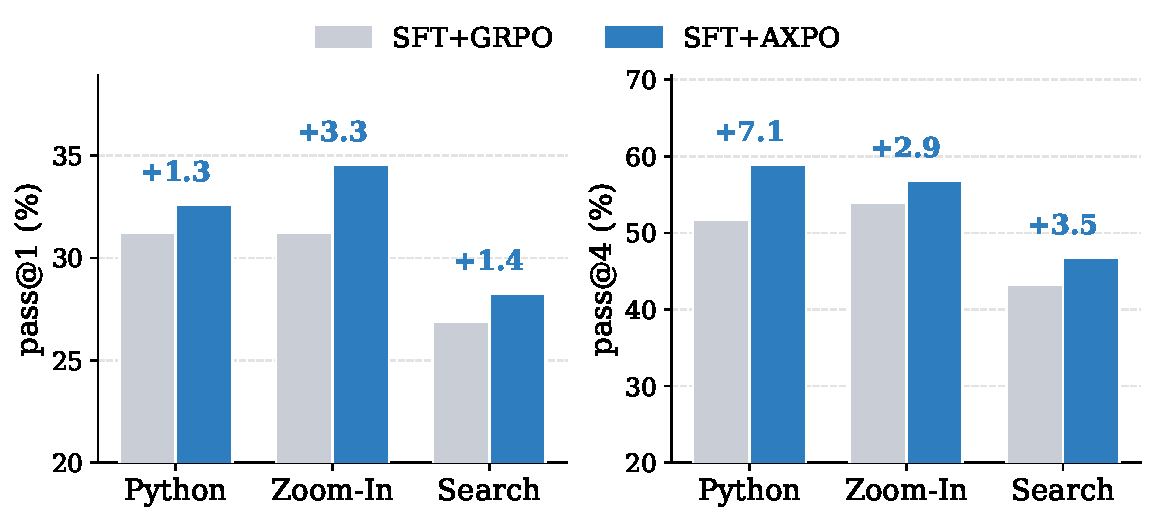
\includegraphics[width=\linewidth]{figures/figx_tool_call_quality.pdf}
        \vspace{-0.15in}
        \caption{Per-tool quality on the matched-tool-use subset (questions where both SFT+GRPO and SFT+AXPO invoke the tool). AXPO improves pass@1 and pass@4 across all three tool families.}
        \label{fig:per-tool-quality}
    \end{subfigure}
    \vspace{-0.05in}
    \caption{\textbf{Post-training analysis} pooled over MathVision, VisualProbe-Hard, and HR-MMSearch on 8B model. Conditional Pass@1 is measured on 715 tool-attempted questions from each benchmark.}
    \vspace{-0.2in}
    \label{fig:matched-analysis}
\end{figure}
